\vspace{-5pt}
\section{Experiments}

\begin{table*}[t]
    \centering
    \small
    
    \begin{tabular}{c|clccccccc}
        \toprule
      General Arch.  &  Token Mixer    & Outcome Model    & Image Size & Params (M)  & MACs (G) & Top-1 (\%) \\
        \whline
    {\multirow{5}{*}{\makecell[c]{Convolutional \\ Neural Netowrks}}}  & \multirow{5}{*}{---}   & \resnetdot{} RSB-ResNet-18 \cite{resnet, resnet_improved} & 224 & 12 & 1.8 & 70.6 \\
         &   & \resnetdot{} RSB-ResNet-34 \cite{resnet, resnet_improved} & 224 & 22 & 3.7 & 75.5 \\
         &   & \resnetdot{} RSB-ResNet-50 \cite{resnet, resnet_improved} & 224 & 26 & 4.1 & 79.8 \\
         &   & \resnetdot{} RSB-ResNet-101 \cite{resnet, resnet_improved} & 224 &  45 & 7.9 & 81.3 \\
         &   & \resnetdot{} RSB-ResNet-152 \cite{resnet, resnet_improved} & 224 & 60 & 11.6 & 81.8 \\
        \hline
         
   \multirow{22}{*}{MetaFormer}  & \multirow{8}{*}{Attention} & \vitdot{} ViT-B/16$^*$ \cite{vit} & 224 &  86 & 17.6 & 79.7 \\
             &          & \vitdot{} ViT-L/16$^*$ \cite{vit} & 224 & 307 & 63.6 & 76.1 \\
             &          & \deitdot{} DeiT-S \cite{deit} & 224 & 22 & 4.6 & 79.8 \\
             &          & \deitdot{} DeiT-B \cite{deit} & 224 &  86 & 17.5 & 81.8 \\
             &          & \pvtdot{} PVT-Tiny \cite{pvt} & 224 & 13 & 1.9 & 75.1 \\
             &          & \pvtdot{} PVT-Small \cite{pvt} & 224 & 25 & 3.8 & 79.8 \\
             &          & \pvtdot{} PVT-Medium \cite{pvt} & 224 & 44 &  6.7 & 81.2 \\
             &          & \pvtdot{} PVT-Large \cite{pvt} & 224 & 61 &  9.8 & 81.7 \\
    \cline{2-7}
             & \multirow{9}{*}{Spatial MLP} & \mlpmixerdot{} MLP-Mixer-B/16 \cite{mlp-mixer} & 224 & 59 & 12.7 & 76.4 \\
             &             & \resmlp{} ResMLP-S12 \cite{resmlp} & 224 & 15 & 3.0 & 76.6 \\
             &             & \resmlp{} ResMLP-S24 \cite{resmlp} & 224 & 30 & 6.0 & 79.4 \\
             &             & \resmlp{} ResMLP-B24 \cite{resmlp} & 224 & 116 & 23.0 & 81.0 \\
             &             & \swinmixer{} Swin-Mixer-T/D24 \cite{swin} & 256 & 20 & 4.0 & 79.4 \\
             &             & \swinmixer{} Swin-Mixer-T/D6 \cite{swin} & 256 & 23 & 4.0 & 79.7 \\
             &             & \swinmixer{} Swin-Mixer-B/D24 \cite{swin} & 224 & 61 & 10.4 & 81.3 \\
             &             & \gmlp{} gMLP-S \cite{gmlp} & 224 & 20 & 4.5 & 79.6 \\
             &             & \gmlp{} gMLP-B \cite{gmlp} & 224 & 73 & 15.8 & 81.6 \\
    \cline{2-7}
             & \multirow{5}{*}{Pooling}  & \poolformer{} PoolFormer-S12 & 224 & 12 & 1.8 & 77.2 \\ % 77.3
             &         & \poolformer{} PoolFormer-S24 & 224 & 21 & 3.4 & 80.3 \\
             &         & \poolformer{} PoolFormer-S36 & 224 & 31 & 5.0 & 81.4 \\ % 81.5
             &         & \poolformer{} PoolFormer-M36 & 224 & 56 & 8.8 & 82.1 \\
             &         & \poolformer{} PoolFormer-M48 & 224 & 73 & 11.6 & 82.5 \\
    \bottomrule
             
    \end{tabular}
    \vspace{-3mm}
    \caption{
    \textbf{Performance of different types of models on ImageNet-1K  classification.} 
    All these models are only trained on the ImageNet-1K training set and the accuracy on the validation set is reported. RSB-ResNet means the results are from ``ResNet Strikes Back" \cite{resnet_improved} where ResNet \cite{resnet} is trained with improved training procedure for 300 epochs. $^*$ denotes results of ViT trained with extra regularization from \cite{mlp-mixer}. The numbers of MACs of PoolFormer are counted by \texttt{fvcore} \cite{fvcore} library.
    \label{tab:imagenet}}
    \vspace{-2mm}
\end{table*}

%%%%%%%%% Figure: MetaFormer performance full plot
\begin{figure*}[t]
  \centering
   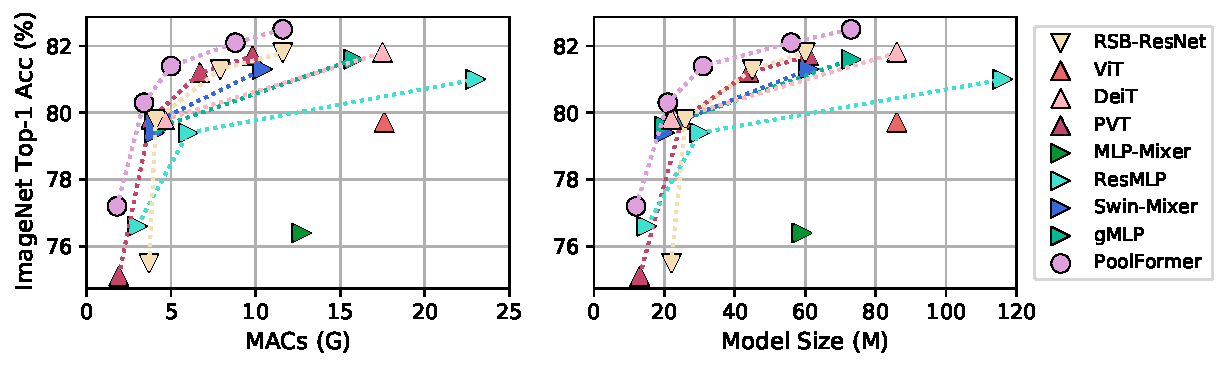
\includegraphics[width=0.95\linewidth]{figures/MetaFormer_full_plot.pdf}
   \vspace{-4mm}
   \caption{\textbf{ImageNet-1K validation accuracy \vs MACs/Model Size.} RSB-ResNet means the results are from ``ResNet Strikes Back" \cite{resnet_improved} where ResNet \cite{resnet} is trained with improved training procedure for 300 epochs.}
   \label{fig:overall_comparision}
\vspace{-1mm}
\end{figure*}


\subsection{Image classification}
\myPara{Setup} 
ImageNet-1K \cite{imagenet} is one of the most widely used datasets in computer vision. It contains about 1.3M training images and 50K validation images, covering common 1K classes. Our training scheme mainly follows \cite{deit} and \cite{cait}. Specifically, MixUp \cite{mixup}, CutMix \cite{cutmix}, CutOut \cite{cutout} and RandAugment \cite{randaugment} are used for data augmentation. The models are trained for 300 epochs using AdamW optimizer \cite{adam, adamw} with weight decay $0.05$ and peak learning rate $\mathrm{lr} = 1e^{-3} \cdot \mathrm{batch\ size} / 1024$ (batch size 4096 and learning rate $4e^{-3}$ are used in this paper). The number of warmup epochs is 5 and cosine schedule is used to decay the learning rate. Label Smoothing \cite{label_smoothing} is set as 0.1. Dropout is disabled but stochastic depth \cite{stochastic_depth} and LayerScale \cite{cait} are used to help train deep models. 
We modified Layer Normalization \cite{layer_norm} to compute the mean and variance along token and channel dimensions compared to only channel dimension in vanilla Layer Normalization. Modified Layer Normalization (MLN) can be implemented for channel-first data format with GroupNorm API in PyTorch by specifying the group number as 1. MLN is preferred by PoolFormer as shown in Section \ref{sec:ablation}. See the appendix for more details on hyper-parameters. Our implementation is based on the \texttt{Timm} codebase \cite{timm} and the experiments are run on TPUs. 


\myPara{Results} 
Table \ref{tab:imagenet} shows the performance of PoolFormers on ImageNet classification. Qualitative results are shown in the appendix. Surprisingly, despite the simple pooling token mixer, PoolFormers can still achieve highly competitive performance compared with CNNs and other MetaFormer-like models. For example, PoolFormer-S24 reaches the top-1 accuracy of more than 80 while only requiring 21M parameters and 3.4G MACs. Comparatively, the well-established ViT baseline DeiT-S \cite{deit}, attains slightly worse accuracy of 79.8 and requires 35\% more MACs (4.6G). To obtain similar accuracy, MLP-like model ResMLP-S24 \cite{resmlp} needs 43\% more parameters (30M) as well as 76\% more computation (6.0G) while only 79.4 accuracy is attained. Even compared with more improved ViT and MLP-like variants \cite{pvt, gmlp}, PoolFormer still shows better performance. Specifically, the pyramid Transformer PVT-Medium obtains 81.2 top-1 accuracy with 44M parameters and 6.7G MACs while PoolFormer-S36 reaches 81.4 with 30\% fewer parameters (31M) and 25\% fewer MACs (5.0G) than those of PVT-Medium. 


Besides, compared with RSB-ResNet (``ResNet Strikes Back") \cite{resnet_improved} where ResNet \cite{resnet} is trained with improved training procedure for the same 300 epochs, PoolFormer still performs better. With $\sim$ 22M parameters/3.7G MACs, RSB-ResNet-34 \cite{resnet_improved} gets 75.5 accuracy while PoolFormer-S24 can obtain 80.3. Since the local spatial modeling ability of the pooling layer is much worse than the neural convolution layer, the competitive performance of PoolFormer can only be attributed to its general architecture MetaFormer.


With the pooling operator,  each token evenly aggregates the features from its nearby tokens. Thus it is an extremely basic token mixing operation. However, the experiment results show that even with this embarrassingly simple token mixer, MetaFormer still obtains highly competitive performance. 
Figure \ref{fig:overall_comparision} clearly shows that PoolFormer surpasses other models with fewer MACs and parameters. 
This finding conveys that the general architecture MetaFormer is actually what we need when designing vision models. By adopting MetaFormer, it is guaranteed that the derived models would have the potential to achieve reasonable performance. 

%%%%%%%%% Table: COCO det
\begin{table*}[t]
\small
\centering
\setlength{\tabcolsep}{2pt}
% Please add the following required packages to your document preamble:
% \usepackage{booktabs}
% \usepackage{graphicx}
% \usepackage[table,xcdraw]{xcolor}
% If you use beamer only pass "xcolor=table" option, i.e. \documentclass[xcolor=table]{beamer}
\begin{table*}
% \vspace{-0.05in}
\centering
\resizebox{.9\linewidth}{!}{%
\setlength{\tabcolsep}{5pt}
\begin{tabular}{lccccccccc}
\toprule
Backbone &
\begin{tabular}[c]{c}Params \\ (M)\end{tabular} &
\begin{tabular}[c]{c}FLOPs \\ (G)\end{tabular} &
\begin{tabular}[c]{c}Latency on\\GPU (ms)\end{tabular} &
\hspace{0.1cm} $AP^b$ \hspace{0.1cm}&
\hspace{0.1cm} $AP^b_{50}$ \hspace{0.1cm}&
\hspace{0.1cm} $AP^b_{75}$ \hspace{0.1cm}&
\hspace{0.1cm} $AP^m$ \hspace{0.1cm}&
\hspace{0.1cm} $AP^m_{50}$ \hspace{0.1cm}&
\hspace{0.1cm} $AP^m_{75}$ \hspace{0.1cm} \\ \midrule
ResNet50~\cite{he2016deep}        & 44.2  & 253   & 54.9  & 38.0 & 58.6 & 41.4 & 34.4 & 55.1 & 36.7 \\
PoolFormer-S24~\cite{yu2022metaformer}    & 41.0  & 233   & 111.0 & 40.1 & 62.2 & 43.4 & 37.0 & 59.1 & 39.6 \\
PVT-Small~\cite{wang2021pyramid}        & 44.1  & 238   & 89.5  & 40.4 & 62.9 & 43.8 & 37.8 & 60.1 & 40.3 \\
\cc FasterNet-S      &\cc 49.0  &\cc 258   &\cc 54.3  &\cc 39.9 &\cc 61.2 &\cc 43.6 &\cc 36.9 &\cc 58.1 &\cc 39.7 \\ \midrule
ResNet101~\cite{he2016deep}       & 63.2  & 329   & 68.9  & 40.4 & 61.1 & 44.2 & 36.4 & 57.7 & 38.8 \\
ResNeXt101-32$\times$4d~\cite{xie2017aggregated} & 62.8  & 333   & 80.5  & 41.9 & 62.5 & 45.9 & 37.5 & 59.4 & 40.2 \\
PoolFormer-S36~\cite{yu2022metaformer}    & 50.5  & 266   & 146.9 & 41.0 & 63.1 & 44.8 & 37.7 & 60.1 & 40.0 \\
PVT-Medium~\cite{wang2021pyramid}       & 63.9  & 295   & 117.3 & 42.0 & 64.4 & 45.6 & 39.0 & 61.6 & 42.1 \\
\cc FasterNet-M      &\cc 71.2  &\cc 344   &\cc 71.4  &\cc 43.0 &\cc 64.4 &\cc 47.4 &\cc 39.1 &\cc 61.5 &\cc 42.3 \\ \midrule
ResNeXt101-64$\times$4d~\cite{xie2017aggregated} & 101.9 & 487   & 112.9 & 42.8 & 63.8 & 47.3 & 38.4 & 60.6 & 41.3 \\
PVT-Large~\cite{wang2021pyramid}        & 81.0  & 358   & 152.2 & 42.9 & 65.0 & 46.6 & 39.5 & 61.9 & 42.5 \\
\cc FasterNet-L      &\cc 110.9 &\cc 484 &\cc 93.8  &\cc 44.0 &\cc 65.6 &\cc 48.2 &\cc 39.9 &\cc 62.3 &\cc 43.0 \\ \bottomrule
\end{tabular}%
}
\vspace{-0.08in}
\caption{Results on COCO object detection and instance segmentation benchmarks. FLOPs are calculated with image size (1280, 800).}
\label{tab:coco}
\vspace{-0.1in}
\end{table*}
\vspace{-3mm}
\caption{\textbf{Performance of object detection using RetinaNet, and object detection and instance segmentation using Mask R-CNN on COCO \texttt{val2017}~\cite{coco}.} $1 \times$ training schedule (\ie 12 epochs) is used for training detection models. $AP^b$ and $AP^m$ represent bounding box AP and mask AP, respectively.}
\label{tab:coco_det} 
\vspace{-3mm}
\end{table*}


%%%%%%%%% Table: COCO det and ins seg
\begin{comment}
\begin{table*}[t]
\centering
\setlength{\tabcolsep}{10pt}
\input{tables/coco_det_seg}
\vspace{-2mm}
\caption{\textbf{Performance of object detection and instance segmentation on COCO \texttt{val2017} \cite{coco}}. $AP^b$ and $AP^m$ represent bounding box AP and mask AP, respectively. All models are based on Mask R-CNN and trained by $1 \times$ training schedule (\ie 12 epochs).}
\label{tab:coco_det_seg} 
\end{table*}
\end{comment}


%%%%%%%%% Table: ADE20K
\begin{table}[t]
\small
\centering
\setlength{\tabcolsep}{3.5pt}
\begin{tabular}{l|c|c}
\toprule
\multirow{2}{*}{Backbone} & \multicolumn{2}{c}{Semantic FPN}\\
\cline{2-3}
& Params (M) & mIoU (\%) \\
    \whline
	\resnetdot{} ResNet-18~\cite{resnet}                & 15.5 &  32.9 \\
	\pvtdot{} PVT-Tiny~\cite{pvt}           & 17.0 &  35.7 \\
	\poolformer{} PoolFormer-S12                    & 15.7 &  37.2 \\
	\hline
    \resnetdot{} ResNet-50~\cite{resnet}                & 28.5 &  36.7 \\
    \pvtdot{} PVT-Small~\cite{pvt}          & 28.2 &  39.8 \\
	\poolformer{} PoolFormer-S24                    & 23.2 &  40.3 \\
    \hline
    \resnetdot{} ResNet-101~\cite{resnet}               & 47.5 &  38.8\\
    \resnetdot{} ResNeXt-101-32x4d~\cite{xie2017aggregated} & 47.1 &  39.7 \\
    \pvtdot{} PVT-Medium~\cite{pvt}         & 48.0 & 41.6 \\
    \poolformer{} PoolFormer-S36                    & 34.6 & 42.0 \\
    \hline
    \pvtdot{} PVT-Large~\cite{pvt}          & 65.1 &  42.1 \\
    \poolformer{} PoolFormer-M36                    & 59.8 & 42.4 \\
    \hline
    \resnetdot{} ResNeXt-101-64x4d~\cite{xie2017aggregated} & 86.4 &  40.2 \\
    \poolformer{} PoolFormer-M48                   & 77.1 &  42.7 \\
\bottomrule
\end{tabular}
\vspace{-3mm}
\caption{\textbf{Performance of Semantic segmentation on ADE20K~\cite{ade20k} validation set.} All models are equipped with Semantic FPN~\cite{fpn}.}
\label{tab:ade20k}
\normalsize
\vspace{-5mm}
\end{table}


\subsection{Object detection and instance segmentation}
\vspace{-1pt}
\myPara{Setup} We evaluate PoolFormer on the challenging COCO benchmark \cite{coco} that includes 118K training images (\texttt{train2017}) and 5K validation images (\texttt{val2017}). The models are trained on training set and the performance on validation set is reported. PoolFormer is employed as the backbone for two standard detectors, \ie, RetinaNet~\cite{retinanet} and Mask R-CNN~\cite{mask_rcnn}. ImageNet pre-trained weights are utilized to initialize the backbones and Xavier \cite{glorot2010understanding} to initialize the added layers. AdamW~\cite{adam, adamw}  is adopted for training with an initial learning rate of $1\times10^{-4}$ and batch size of 16. Following \cite{retinanet, mask_rcnn}, we employ 1$\times$ training schedule, \ie, training the detection models for 12 epochs. The training images are resized into shorter side of 800 pixels and longer side of no more than 1,333 pixels. For testing, the shorter side of the images is also resized to 800 pixels. The implementation is based on the \texttt{mmdetection} \cite{mmdetection} codebase and the experiments are run on 8 NVIDIA A100 GPUs. 

\myPara{Results}
Equipped with RetinaNet for object detection, PoolFormer-based models consistently outperform their comparable ResNet counterparts as shown in Table \ref{tab:coco_det}. For instance, PoolFormer-S12 achieves 36.2 AP, largely surpassing that of ResNet-18 (31.8 AP). 
Similar results are observed for those models based on Mask R-CNN on object detection and instance segmentation. For example, PoolFormer-S12 largely surpasses ResNet-18 (bounding box AP 37.3 \vs 34.0, and mask AP 34.6 \vs 31.2). 
Overall, for COCO object detection and instance segmentation, PoolForemrs achieve competitive performance, consistently outperforming those counterparts of ResNet. 


%%%%%%%%% Table: Ablation
\begin{table*}[t]
\small
\centering
\setlength{\tabcolsep}{2pt}
% \scalebox{0.85}{% Please add the following required packages to your document preamble:
% \usepackage{booktabs}
% \usepackage{multirow}
\begin{table}
\centering
% \vspace{-0.05in}
\resizebox{1.\linewidth}{!}{%
\setlength{\tabcolsep}{1pt}
\begin{tabular}{llcccc}
\toprule
Ablation&
Variant &
\begin{tabular}[c]{@{}c@{}} {\small Throughput}  \\ on {\small GPU} \\ (fps)\end{tabular} &
\begin{tabular}[c]{@{}c@{}} {\small Latency} \\ on {\small CPU} \\ (ms)\end{tabular} &
\begin{tabular}[c]{@{}c@{}} {\small Latency} \\ on {\small ARM} \\ (ms)\end{tabular} &
\begin{tabular}[c]{@{}c@{}}Acc. \\ (\%)\end{tabular} \\ \midrule
\multirow{3}{*}{Partial ratio} & $\text{T0}^*$ w/  $r = 1/2$   &6626       & 9.6       & 145       & 71.7      \\
                               &\cc T0 w/ $r = 1/4$ &\cc 6807   &\cc 9.2    &\cc 143    &\cc 71.9   \\
                               & $\text{T0}^*$ w/ $r = 1/8$    &6204	     &8.9        &140        & 71.3    \\ \midrule
\multirow{2}{*}{Normalization} &\cc T0 w/ BN          &\cc 6807   &\cc 9.2    &\cc 143 &\cc 71.9                   \\
                               & T0 w/ LN          &5515	  &10.7 &159                         & 71.9                     \\ \midrule
\multirow{5}{*}{Activation}    & T0 w/ ReLU        &6929	  &8.2  &114                         & 71.3                     \\
                               &$\text{T0}^*$ w/ ReLU        & 5866                 & 9.3                  & 143 & 71.7 \\
                               &\cc T0 w/ GELU        &\cc 6807   &\cc 9.2    &\cc 143 &\cc 71.9                     \\
                               &\cc T2 w/ ReLU        &\cc 1991                 &\cc 33.5                 &\cc 497 &\cc 78.9                     \\
                               & T2 w/ GELU        &1985	  &35.4  &557                         & 78.7 \\ 
\bottomrule
\end{tabular}%
}
\vspace{-0.1in}
\caption{Ablation on the partial ratio, normalization, and activation of FasterNet. Rows highlighted in grey are the default settings. $\text{T0}^*$ denotes T0 variants with modified network width and depth.}
\label{tab:ablation}
\vspace{-0.1in}
\end{table}
}
% Please add the following required packages to your document preamble:
% \usepackage{booktabs}
% \usepackage{multirow}
\begin{table}
\centering
% \vspace{-0.05in}
\resizebox{1.\linewidth}{!}{%
\setlength{\tabcolsep}{1pt}
\begin{tabular}{llcccc}
\toprule
Ablation&
Variant &
\begin{tabular}[c]{@{}c@{}} {\small Throughput}  \\ on {\small GPU} \\ (fps)\end{tabular} &
\begin{tabular}[c]{@{}c@{}} {\small Latency} \\ on {\small CPU} \\ (ms)\end{tabular} &
\begin{tabular}[c]{@{}c@{}} {\small Latency} \\ on {\small ARM} \\ (ms)\end{tabular} &
\begin{tabular}[c]{@{}c@{}}Acc. \\ (\%)\end{tabular} \\ \midrule
\multirow{3}{*}{Partial ratio} & $\text{T0}^*$ w/  $r = 1/2$   &6626       & 9.6       & 145       & 71.7      \\
                               &\cc T0 w/ $r = 1/4$ &\cc 6807   &\cc 9.2    &\cc 143    &\cc 71.9   \\
                               & $\text{T0}^*$ w/ $r = 1/8$    &6204	     &8.9        &140        & 71.3    \\ \midrule
\multirow{2}{*}{Normalization} &\cc T0 w/ BN          &\cc 6807   &\cc 9.2    &\cc 143 &\cc 71.9                   \\
                               & T0 w/ LN          &5515	  &10.7 &159                         & 71.9                     \\ \midrule
\multirow{5}{*}{Activation}    & T0 w/ ReLU        &6929	  &8.2  &114                         & 71.3                     \\
                               &$\text{T0}^*$ w/ ReLU        & 5866                 & 9.3                  & 143 & 71.7 \\
                               &\cc T0 w/ GELU        &\cc 6807   &\cc 9.2    &\cc 143 &\cc 71.9                     \\
                               &\cc T2 w/ ReLU        &\cc 1991                 &\cc 33.5                 &\cc 497 &\cc 78.9                     \\
                               & T2 w/ GELU        &1985	  &35.4  &557                         & 78.7 \\ 
\bottomrule
\end{tabular}%
}
\vspace{-0.1in}
\caption{Ablation on the partial ratio, normalization, and activation of FasterNet. Rows highlighted in grey are the default settings. $\text{T0}^*$ denotes T0 variants with modified network width and depth.}
\label{tab:ablation}
\vspace{-0.1in}
\end{table}

\vspace{-3mm}
\caption{\textbf{Ablation for PoolFormer on ImageNet-1K classification benchmark.} PoolFormer-S12 is utilized as the baseline to conduct ablation study. The top-1 accuracy on the validation set is reported. $^*$This token mixer utilizes global random matrix $W_R\in \mathbb{R}^{N\times N}$ (parameters are frozen after random initialization) to conduct token mixing by $X'=W_RX$ where $X\in \mathbb{R}^{N \times C}$ are input tokens with the token length of $N$ and channel dimension of $C$. $^\dag$Modified Layer Normalization (MLN) computes the mean and variance along token and channel dimensions compared with vanilla Layer Normalization only along channel dimension. MLN can be implemented with GroupNorm API in PyTorch by specifying the group number equal to 1. The numbers of MACs are counted by \texttt{fvcore} \cite{fvcore} library.
}
\label{tab:ablation}
\normalsize
\vspace{-2mm}
\end{table*}


\vspace{-1pt}
\subsection{Semantic segmentation}
\vspace{-3pt}
\myPara{Setup} 
ADE20K~\cite{ade20k}, a challenging scene parsing benchmark, is selected to evaluate the models for semantic segmentation. The dataset includes 20K and 2K images in the training and validation set, respectively, covering 150 fine-grained semantic categories. PoolFormers are evaluated as backbones equipped with Semantic FPN~\cite{fpn}. ImageNet-1K trained checkpoints are used to initialize the backbones while Xavier~\cite{glorot2010understanding} is utilized to initialize other newly added layers. Common practices~\cite{fpn,chen2017deeplab} train models for 80K iterations with a batch size of 16. To speed up training, we double the batch size to 32 and decrease the iteration number to 40K. The AdamW \cite{adam, adamw} is employed with an initial learning rate of $2\times 10^{-4}$ that will decay in the polynomial decay schedule with a power of 0.9. Images are resized and cropped into $512\times 512$ for training and are resized to shorter side of 512 pixels for testing. Our implementation is based on the \texttt{mmsegmentation} \cite{mmseg2020} codebase and the experiments are conducted on 8 NVIDIA A100 GPUs. 


\myPara{Results} Table~\ref{tab:ade20k} shows the ADE20K semantic segmentation performance of different backbones using FPN~\cite{fpn}. PoolFormer-based models consistently outperform the models with backbones of CNN-based ResNet~\cite{resnet} and ResNeXt \cite{xie2017aggregated} as well as Transformer-based PVT. For instance, PoolFormer-12 achieves mIoU of 37.1, 4.3 and 1.5 better than ResNet-18 and PVT-Tiny, respectively. 


These results demonstrate that our PoorFormer which serves as backbone can attain competitive performance on semantic segmentation although it only utilizes pooling for basically communicating information among tokens. This further indicates the great potential of MetaFormer and supports our claim that MetaFormer is actually what we need.


\subsection{Ablation studies}
\label{sec:ablation}
The experiments of ablation studies are conducted on ImageNet-1K \cite{imagenet}.
Table \ref{tab:ablation} reports the ablation study of PoolFormer. 
We discuss the ablation below according to the following aspects. 


\myPara{Token mixers} Compared with Transformers, the main change made by PoolFormer is using simple pooling as a token mixer. We first conduct ablation for this operator by directly replacing pooling with identity mapping. Surprisingly, MetaFormer with identity mapping can still achieve 74.3\% top-1 accuracy, supporting the claim that MetaFormer is actually what we need to guarantee reasonable performance.


Then the pooling is replaced with global random matrix $W_R\in \mathbb{R^{N\times N}}$ for each block. The matrix is initialized with random values from a uniform distribution on the interval [0, 1), and then Softmax is utilized to normalize each row. After random initialization, the matrix parameters are frozen and it conducts token mixing by $X'=W_RX$ where $X\in \mathbb{R^{N\times C}}$ are the input token features with the token length of $N$ and channel dimension of $C$. The token mixer of random matrix introduces extra 21M frozen parameters for the S12 model since the token lengths are extremely large at the first stage. Even with such random token mixing method, the model can still achieve reasonable performance of 75.8\% accuracy, 1.5\% higher than that of identity mapping. It shows that MetaFormer can still work well even with random token mixing, not to say with other well-designed token mixers. 


Further, pooling is replaced with Depthwise Convolution \cite{chollet2017xception, mamalet2012simplifying} that has learnable parameters for spatial modeling. Not surprisingly, the derived model still achieve highly competitive performance with top-1 accuracy of 78.1\%, 0.9\% higher than PoolFormer-S12 due to its better local spatial modeling ability. Until now, we have specified multiple token mixers in Metaformer, and all resulted models keep promising results, well supporting the claim that MetaFormer is the key to guaranteeing models' competitiveness. Due to the simplicity of pooling, it is mainly utilized as a tool to demonstrate MetaFormer.


We test the effects of pooling size on PoolFormer. We observe similar performance when pooling sizes are 3,  5, and 7. However, when the pooling size increases to 9, there is an obvious performance drop of 0.5\%.  Thus, we adopt the default pooing size of 3 for PoolFormer. 


\myPara{Normalization} We modify Layer Normalization \cite{layer_norm} into Modified Layer Normalization (MLN) that computes the mean and variance along token and channel dimensions compared with only channel dimension in vanilla Layer Normalization. The shape of learnable affine parameters of MLN keeps the same as that of Layer Normalization, \ie, $\mathbb{R^C}$. MLN can be implemented with GroupNorm API in PyTorch by setting the group number as 1. See the appendix for details. We find PoolFormer prefers MLN with 0.7\% or 0.8\% higher than Layer Normalization or Batch Normalization. Thus, MLN is set as default for PoolFormer. When removing normalization, the model can not be trained to converge well, and its performance dramatically drops to only 46.1\%.


\myPara{Activation} We change GELU \cite{gelu} to ReLU \cite{relu} or SiLU \cite{silu}. When ReLU is adopted for activation, an obvious performance drop of 0.8\% is observed. For SiLU, its performance is almost the same as that of GELU. Thus, we still adopt GELU as default activation. 


\myPara{Other components} Besides token mixer and normalization discussed above, residual connection \cite{resnet} and channel MLP \cite{rosenblatt1961principles, rumelhart1985learning} are two other important components in MetaFormer. Without residual connection or channel MLP, the model cannot converge and only achieves the accuracy of 0.1\%/5.7\%, proving the indispensability of these parts.


\myPara{Hybrid stages} Among token mixers based on pooling, attention, and spatial MLP, the pooling-based one can handle much longer input sequences while attention and spatial MLP are good at capturing global information. 
Therefore, it is intuitive to stack MetaFormers with pooling in the bottom stages to handle long sequences and use attention or spatial MLP-based mixer in the top stages, considering the sequences have been largely shortened. Thus, we replace the token mixer pooling with attention or spatial FC \footnote{Following \cite{resmlp}, we use only one spatial fully connected layer as a token mixer, so we call it FC.} in the top one or two stages in PoolFormer. From Table \ref{tab:ablation}, the hybrid models perform quite well. The variant with pooling in the bottom two stages and attention in the top two stages delivers highly competitive performance. 
It achieves 81.0\% accuracy with only 16.5M parameters and 2.5G MACs. 
As a comparison, ResMLP-B24 needs $7.0\times$ parameters (116M) and $9.2\times$ MACs (23.0G) to achieve the same accuracy. These results indicate that combining pooling with other token mixers for MetaFormer may be a promising direction to further improve the performance. 




